% Chapter 2

\chapter{Heterologous expression of the base unfoldase} % Write in your own chapter title
\label{Chapter2}
\lhead{Chapter 2. \emph{Heterologous expression of the base unfoldase}} % Write in your own chapter title to set the page header


\section{Introduction}



%%-------------------------

\section{Results}

\subsection{Cloning, expression and purification of the base from \textit{S. cerevisiae} in \textit{E. coli}}

The base subcomplex of the proteasome from \textit{Saccharomyces cerevisiae} was produced in \textit{Escherichia coli} by co-expression of thirteen yeast proteins, including nine integral base subunits (Rpt1\---6, Rpn1, Rpn2, Rpn13) and four proteasome assembly chaperones (Nas2, Nas6, Rpn14, Hsm329-32) as depicted in Fig. \ref{fig:vectors}. We isolated assembled base by tandem-affinity purification using tags on two different subunits, followed by gel\---filtration chromatography (Fig. \ref{fig:sizing}). The purified base exhibited appropriate stoichiometry and no subunit truncations, as revealed by SDS\---PAGE (Fig. \ref{fig:basegel}) and mass spectrometry (data not shown, R.B.). We observed Nas6, Hsm3, and Rpn14 stably associated with the recombinant base, whereas these chaperones were not present in the base purified from yeast, as indicated by SDS\---PAGE, size-exclusion chromatography, and native PAGE (Fig. \ref{fig:nativegel}). 

%-------------------------------------------------------
\begin{figure}[t]
\centering
\subfigure{%
	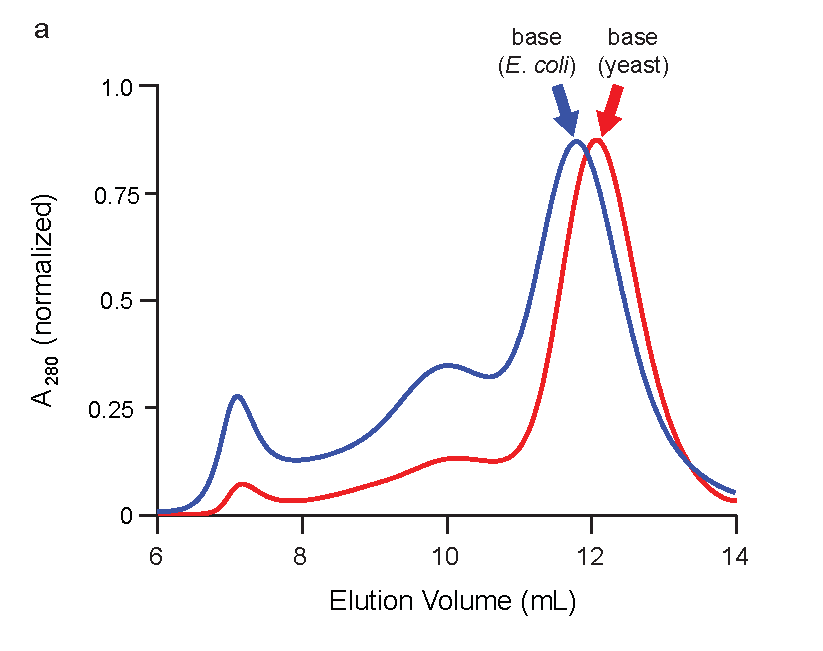
\includegraphics[scale=0.7]{sizing}
	\label{fig:sizing}}
\quad	
\subfigure{%
	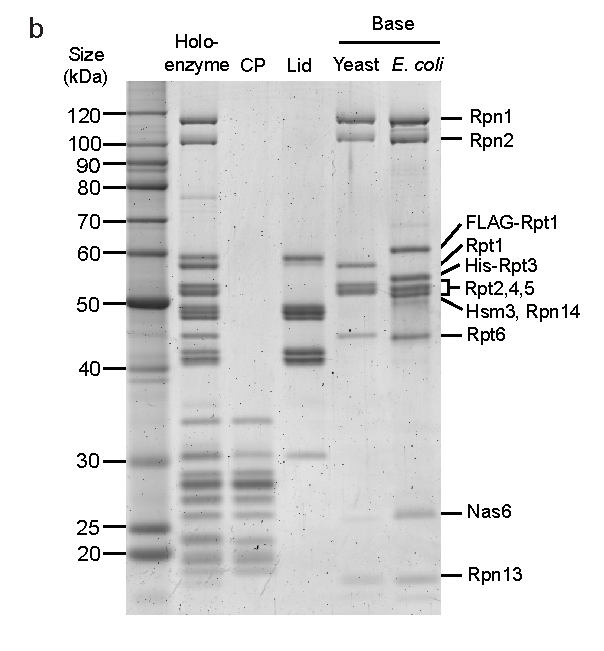
\includegraphics[scale=0.7]{basegel}
	\label{fig:basegel}}
%
\caption[Purification of base and other proteasome subcomplexes]{Purification of base and other proteasome subcomplexes.\par
\textbf{(a)} Sypro\---Ruby stained SDS\---PAGE of the purified proteasomal subcomplexes used in this study. Endogenous complexes were isolated from yeast using FLAG tags on Rpn11 for holoenzyme and lid, on Pre1 for core particle (CP), and on Rpn2 for base preparations. Recombinant base expressed in \textit{E. coli} was purified using a FLAG tag on Rpt1 and a His$_6$ tag on Rpt3. Proteasome chaperones Nas6, Hsm3 and Rpn14 only co\---purify with the base subcomplex produced in \textit{E. coli}. \textbf{(b)} Endogenous (red) and \textit{E. coli}\---expressed, recombinant (blue) base subcomplexes show similar elution profiles from a Superose 6 size\---exclusion column. The slightly smaller elution volume for recombinant base is attributed to the co-purification of proteasome\---specific chaperones that stably associate with the complex when heterologously expressed in the absence of core particle in \textit{E. coli} (Fig. \ref{fig:basegel}). The absorbance at 280 nm is normalized for comparison.  For equal cell mass, recombinant base expression yields approximately 10\---fold more protein than the purification of endogenous base from yeast.
}
\label{fig:basesizing}
\end{figure}
%-------------------------------------------------------

%-------------------------------------------------------
\begin{figure}[h]
\centering
\setlength{\fboxrule}{0pt}
\fbox{%
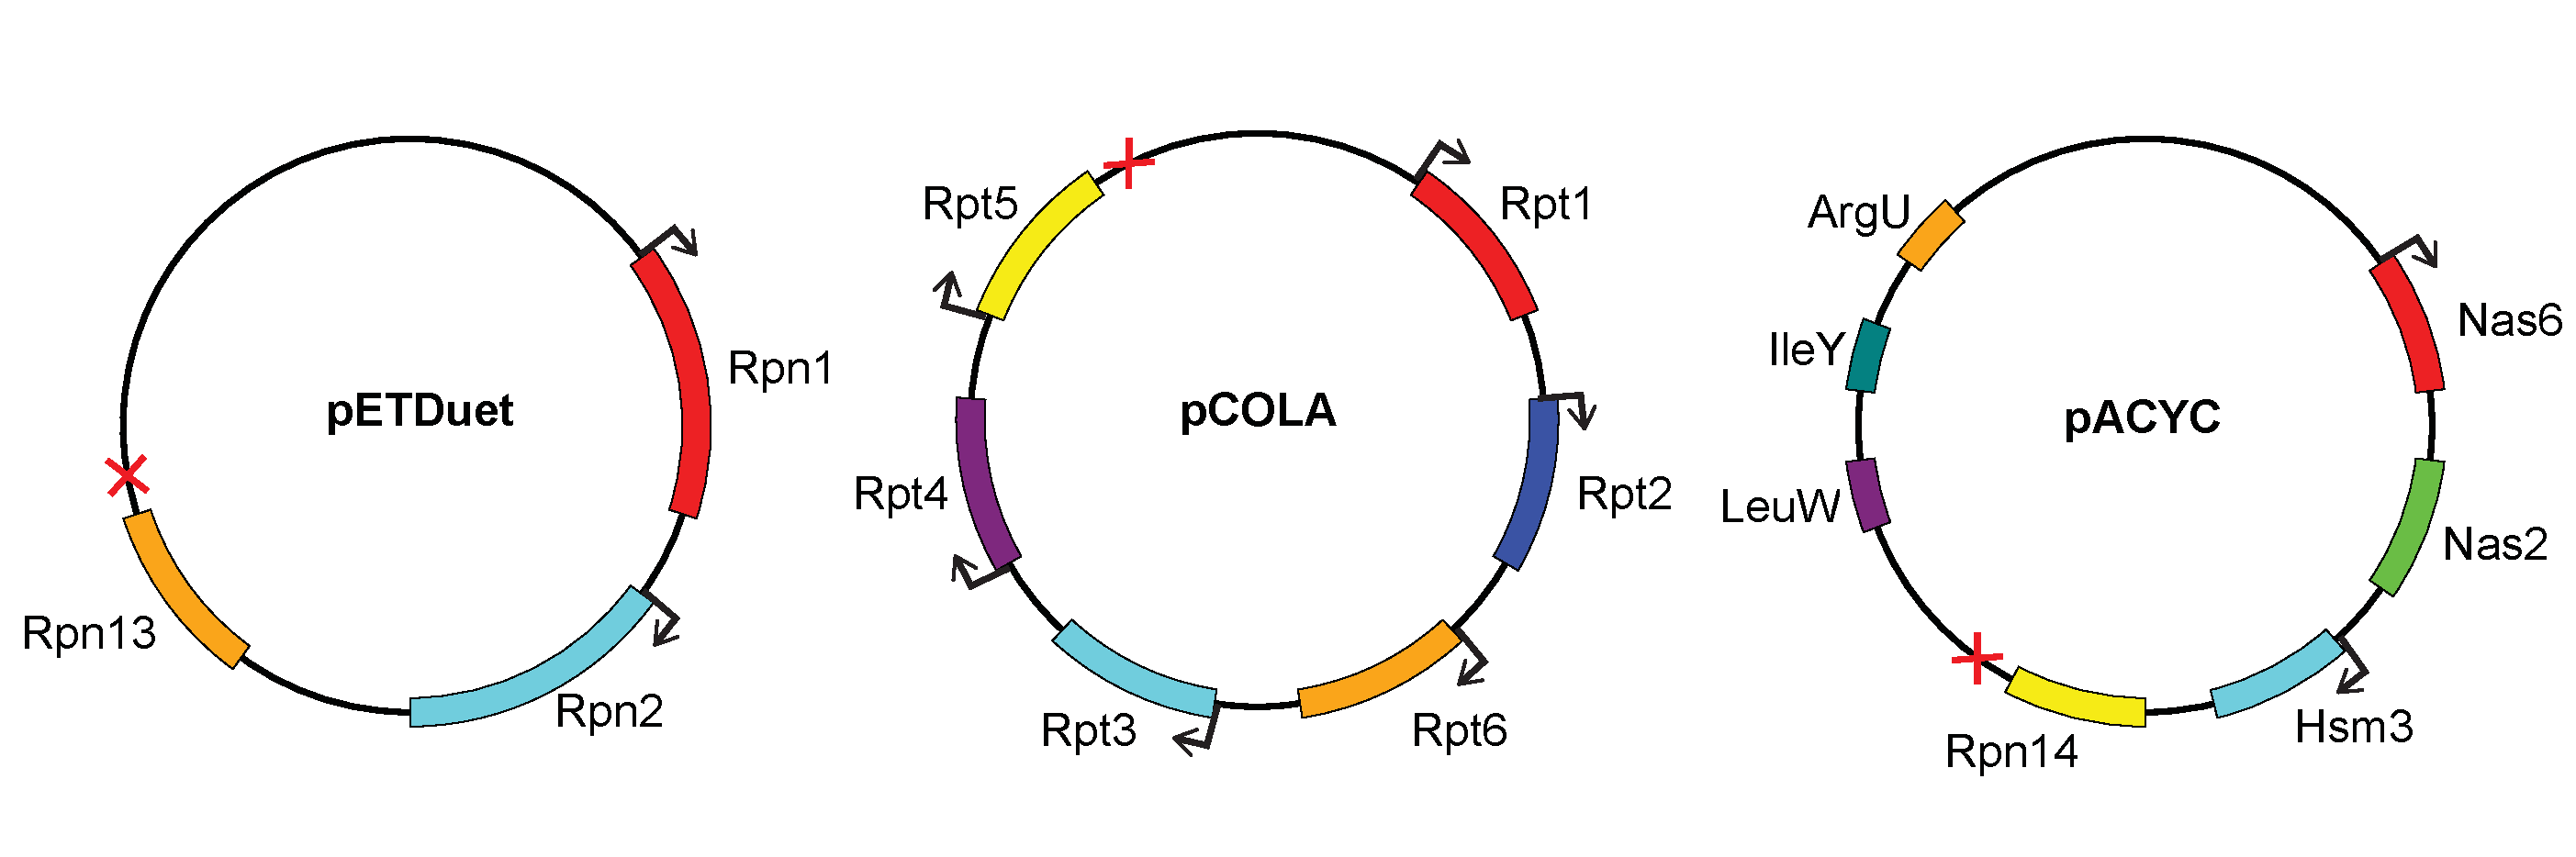
\includegraphics[scale=0.32]{vectors}%
}
\caption[SDS\---PAGE of purified proteasome subcomplexes]{SDS\---PAGE of purified proteasome subcomplexes.\par
Sypro\---Ruby stained SDS\---PAGE of the purified proteasomal subcomplexes used in this study. Endogenous complexes were isolated from yeast using FLAG tags on Rpn11 for holoenzyme and lid, on Pre1 for core particle (CP), and on Rpn2 for base preparations. Recombinant base expressed in \textit{E. coli} was purified using a FLAG tag on Rpt1 and a His$_6$ tag on Rpt3. Proteasome chaperones Nas6, Hsm3 and Rpn14 only co\---purify with the base subcomplex produced in \textit{E. coli} (also see Fig. \ref{fig:gel sizing}).}
\label{fig:vectors}
\end{figure}
%-------------------------------------------------------

%-------------------------------------------------------
\begin{figure}[h]
\centering
\setlength{\fboxrule}{0pt}
\fbox{%
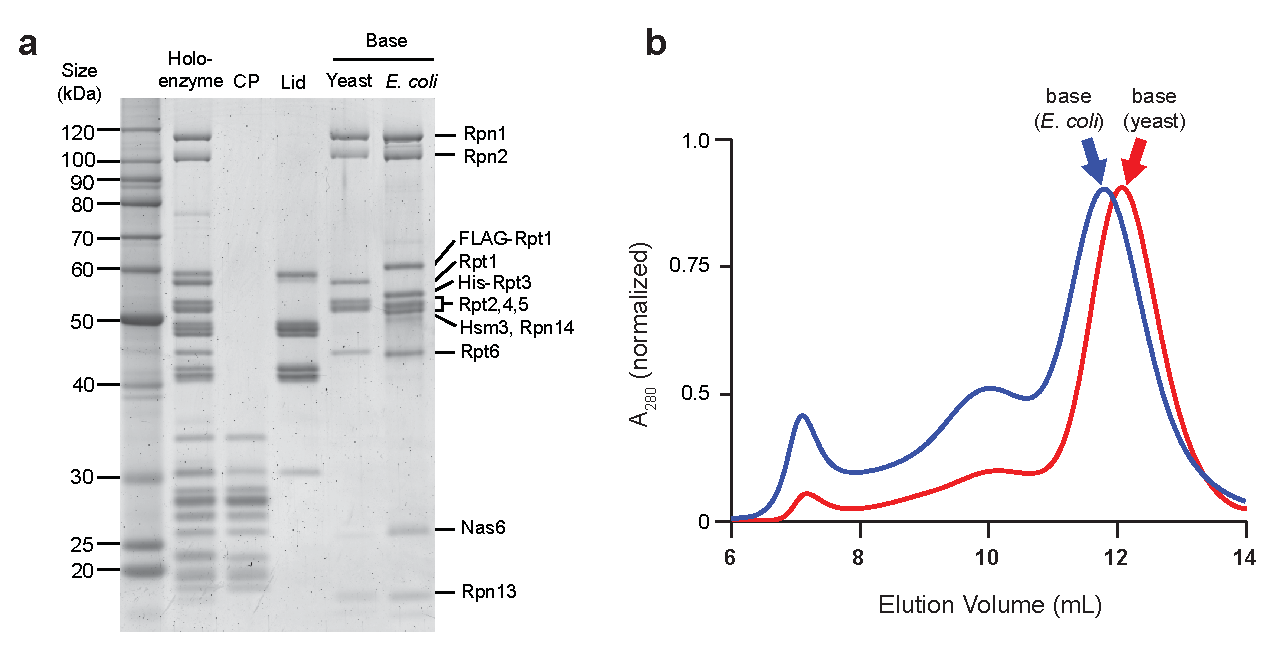
\includegraphics[scale=.7]{gelsizing}%
}
\caption[SDS\---PAGE of purified proteasome subcomplexes]{SDS\---PAGE of purified proteasome subcomplexes.\par
Sypro\---Ruby stained SDS\---PAGE of the purified proteasomal subcomplexes used in this study. Endogenous complexes were isolated from yeast using FLAG tags on Rpn11 for holoenzyme and lid, on Pre1 for core particle (CP), and on Rpn2 for base preparations. Recombinant base expressed in \textit{E. coli} was purified using a FLAG tag on Rpt1 and a His$_6$ tag on Rpt3. Proteasome chaperones Nas6, Hsm3 and Rpn14 only co\---purify with the base subcomplex produced in \textit{E. coli} (also see Fig. \ref{fig:sizing}).}
\label{fig:gelsizing}
\end{figure}
%-------------------------------------------------------

This result is consistent with studies of \textit{in\---vivo} proteasome assembly, indicating that Nas6, Hsm3, and Rpn14 are displaced upon base binding to the core particle and lid, whereas Nas2 dissociates at an earlier stage of base assembly26,29,30,33. One model for \textit{in\---vivo} base assembly proposes that the core particle might act as a template to facilitate the proper arrangement of Rpts in the hexameric ring26. However, our successful production of the base subcomplex in \textit{E. coli} rules out a strict requirement for such templated assembly. \par

\begin{figure}[h]
\centering
\setlength{\fboxrule}{0pt}
\fbox{%
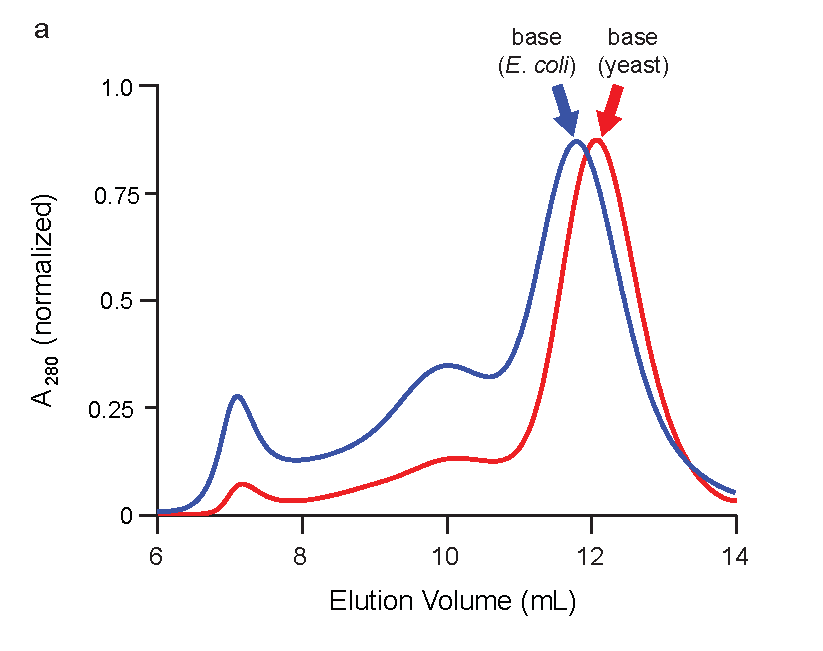
\includegraphics[scale=0.75]{sizing}% 
}
\caption[Size exclusion elution profiles of endogenous and recombinant base]{Size exclusion elution profiles of endogenous and recombinant base.\par
Endogenous (red) and \textit{E. coli}\---expressed, recombinant (blue) base subcomplexes show similar elution profiles from a Superose 6 size\---exclusion column. The slightly smaller elution volume for recombinant base is attributed to the co-purification of proteasome\---specific chaperones that stably associate with the complex when heterologously expressed in the absence of core particle in \textit{E. coli} (Fig. \ref{fig:basegel}). The absorbance at 280 nm is normalized for comparison.  For equal cell mass, recombinant base expression yields approximately 10\---fold more protein than the purification of endogenous base from yeast.}
\label{fig:sizing}
\end{figure}

We compared the activities of the recombinant base to endogenous yeast base. Both base subcomplexes hydrolyzed approximately 51 ATP enz$^{-1}$ min$^{-1}$ in the absence of substrate (Table 1). The ability of the ATP-bound base to interact with core particle and induce gate opening was determined by monitoring the fluorescence increase upon peptidase cleavage of the fluorogenic peptide succinyl\---LLVY\---(7\---amino\---4\---methylcoumarin). In the presence of ATP, recombinant base stimulated core-particle activity approximately 20\---fold, similar to endogenous yeast base. In agreement with previous reports, we measured about two-fold higher peptide hydrolysis with the non\---hydrolysable analog ATP$\gamma$S compared to ATP (unpublished data, R.B.)4,34, which may be due to potential differences in the ATPase\---ring conformation19 or the dynamics of base\---core interactions. 

%nucleotides?

\subsection{Reconstitution of functional 26S proteasome}
%table
%% substrate design? 

\begin{figure}[b]
\centering
\setlength{\fboxrule}{0pt}
\fbox{%
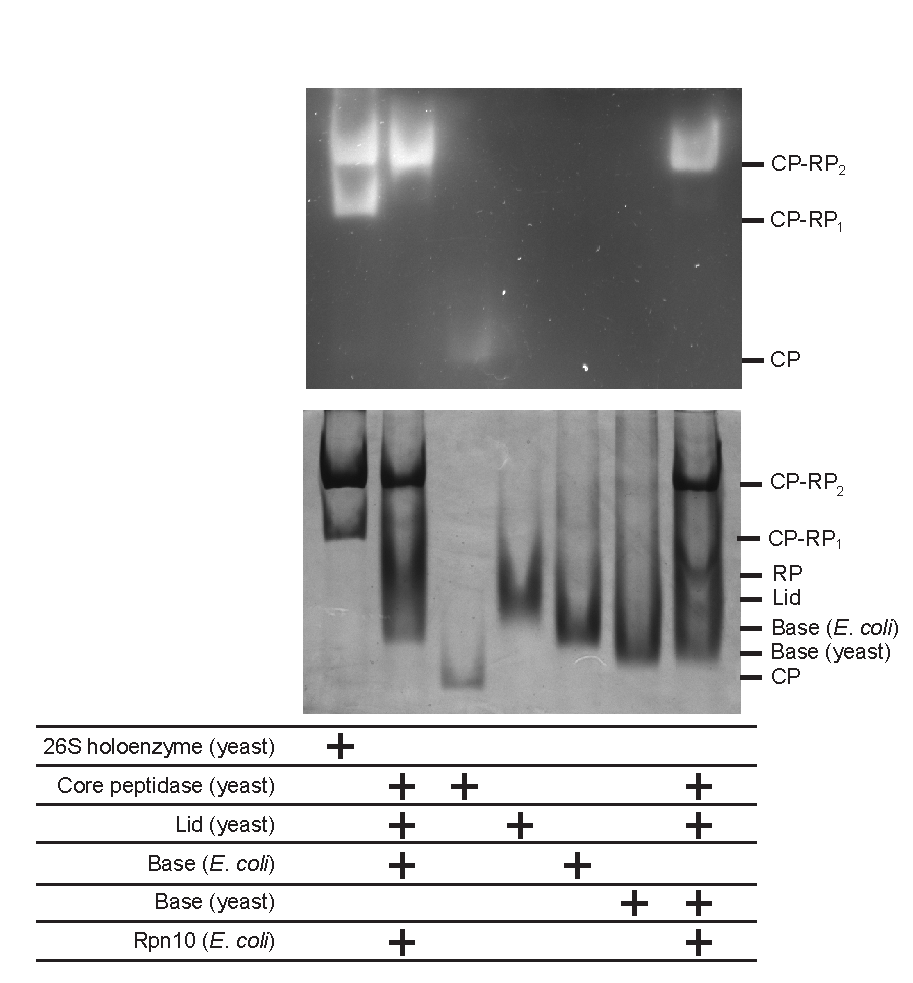
\includegraphics[scale=0.75]{nativegel}% 
}
\caption[Native gel of purified subcomplexes and reconstituted proteasome]{Native gel of purified subcomplexes and reconstituted proteasome.\par
26S holoenzyme reconstituted with CP, lid, Rpn10, and either endogenous or recombinant base was analyzed by native gel electrophoresis. Endogenous yeast 26S holoenzyme and individual CP, lid, and base subcomplexes were also analyzed for comparison. Yeast holoenzyme migrated as two bands corresponding to proteasomes singly (CP\---RP$_1$) and doubly (CP\---RP$_2$) capped with regulatory particles (RP). Excess lid and base was used for reconstituted proteasome samples, which therefore migrated only as doubly capped holoenzyme.}
\label{fig:nativegel}
\end{figure}

\begin{figure}[t]
\centering
\setlength{\fboxrule}{0pt}
\fbox{%
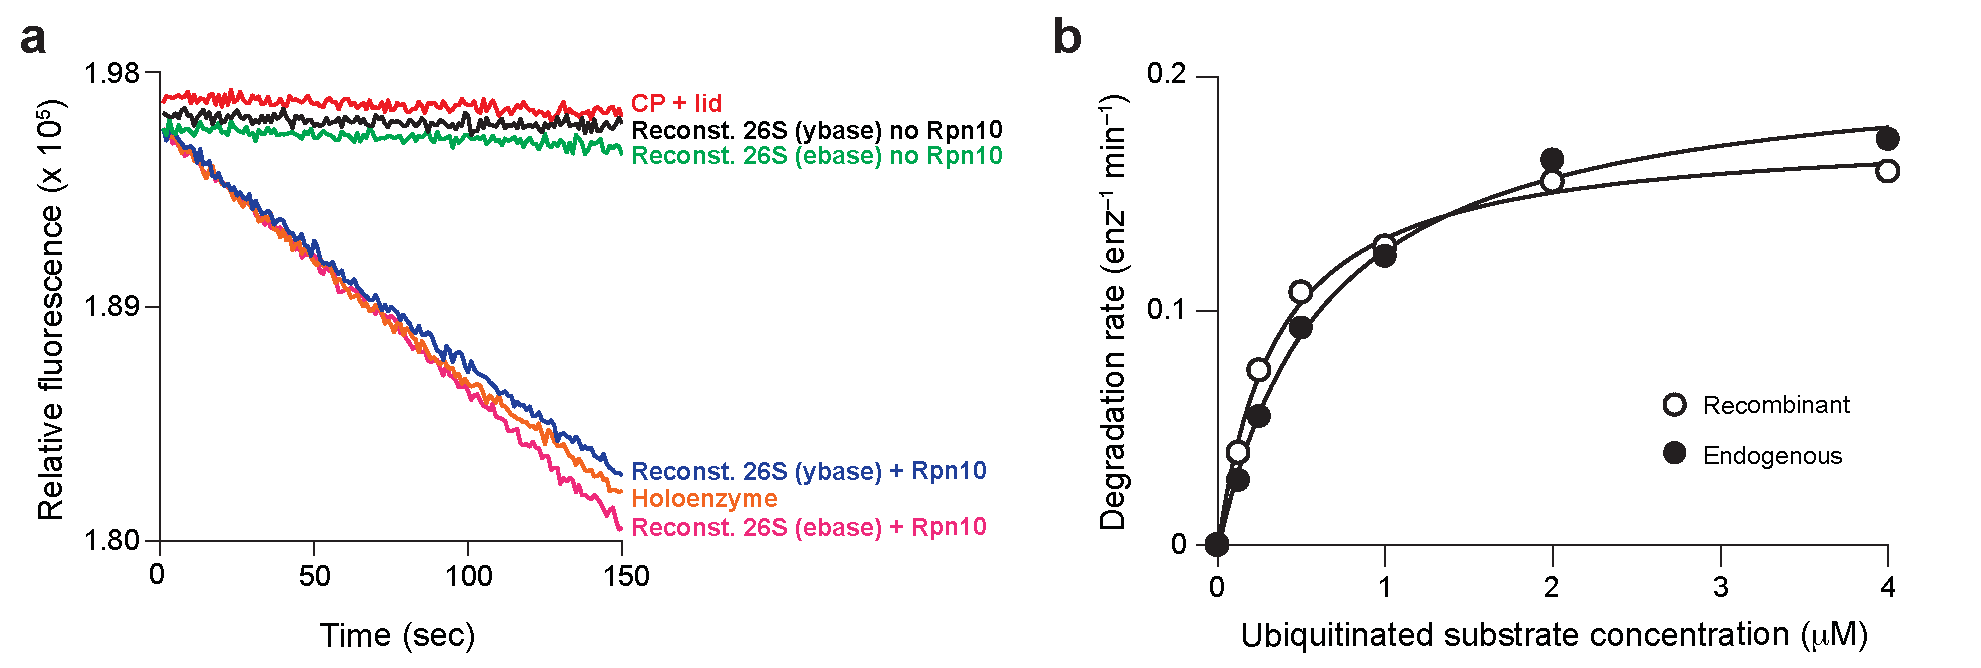
\includegraphics[width=\linewidth]{degcombo}% 
}
\caption[Proteasomal degradation of a fluorescent model substrate]{Proteasomal degradation of a fluorescent model substrate.\par
Degradation of a polyubiquitinated GFP fusion substrate by endogenous yeast holoenzyme or 26S proteasomes reconstituted with saturating recombinant base (ebase) or endogenous yeast base (ybase). Substrate degradation was monitored by the loss of GFP fluorescence and strictly required the addition of Rpn10, despite the presence of Rpn13 (see Fig. \ref{fig:basegel}).

Michaelis\---Menten analyses of substrate degradation by proteasomes reconstituted with endogenous or recombinant base. Degradation reactions were performed using limiting base and excess core particle, lid and Rpn10 to ensure that reconstituted proteasome particles were singly capped. K$_M$ and V$_{max}$ values were 0.63 $\mu$M and 0.21 enz$^{-1}$ min$^{-1}$ for holoenzyme with endogenous base, and 0.35 $\mu$M and 0.18 enz$^{-1}$ min$^{-1}$ for holoenzyme with recombinant base.

}
\label{fig:degcombo}
\end{figure}

Importantly, we also reconstituted 26S holoenzyme, using either endogenous or recombinant base and the lid and core particle purified from yeast. Successful reconstitution was assessed by native PAGE (Fig. \ref{fig:nativegel}) and \textit{in\---vitro} degradation of a polyubiquitinated model substrate, a green fluorescent protein (GFP)\---titin$^{V15P}$\---cyclin\---PY fusion, whose degradation could be measured through the decrease of GFP fluorescence (Fig. \ref{fig:deg}, Fig. \ref{fig:gfpdeg}). Proteasomes reconstituted with saturating recombinant or endogenous base degraded substrate at a maximal rate of 0.3 enz$^{-1}$ min$^{-1}$, comparable to 0.32 enz$^{-1}$ min$^{-1}$ observed for holoenzyme purified from yeast (Table 1). Substrate degradation by reconstituted proteasomes strictly required addition of recombinant Rpn10, an intrinsic ubiquitin\---receptor that does not co\---purify with isolated lid or base subcomplexes. Consistent with previously described degradation defects in the absence of Rpn1035, we found that omitting Rpn10 or deleting its ubiquitin\---interacting motif resulted in 40\---fold slower degradation (Fig. \ref{fig:gfpdeg}, Fig. \ref{fig:degcontrols}), despite the presence of the second ubiquitin receptor, Rpn13. Since proteasome formation did not depend on Rpn10 (data not shown, R.B.) and degradation was not facilitated by Rpn10 lacking its ubiquitin\---interacting motif, this result suggests that Rpn10 is either the primary receptor for our model substrates or required in combination with Rpn13 for multivalent ubiquitin\---chain binding.

\newpage
\vfill

\begin{figure}[p]
\centering
\setlength{\fboxrule}{0pt}
\fbox{%
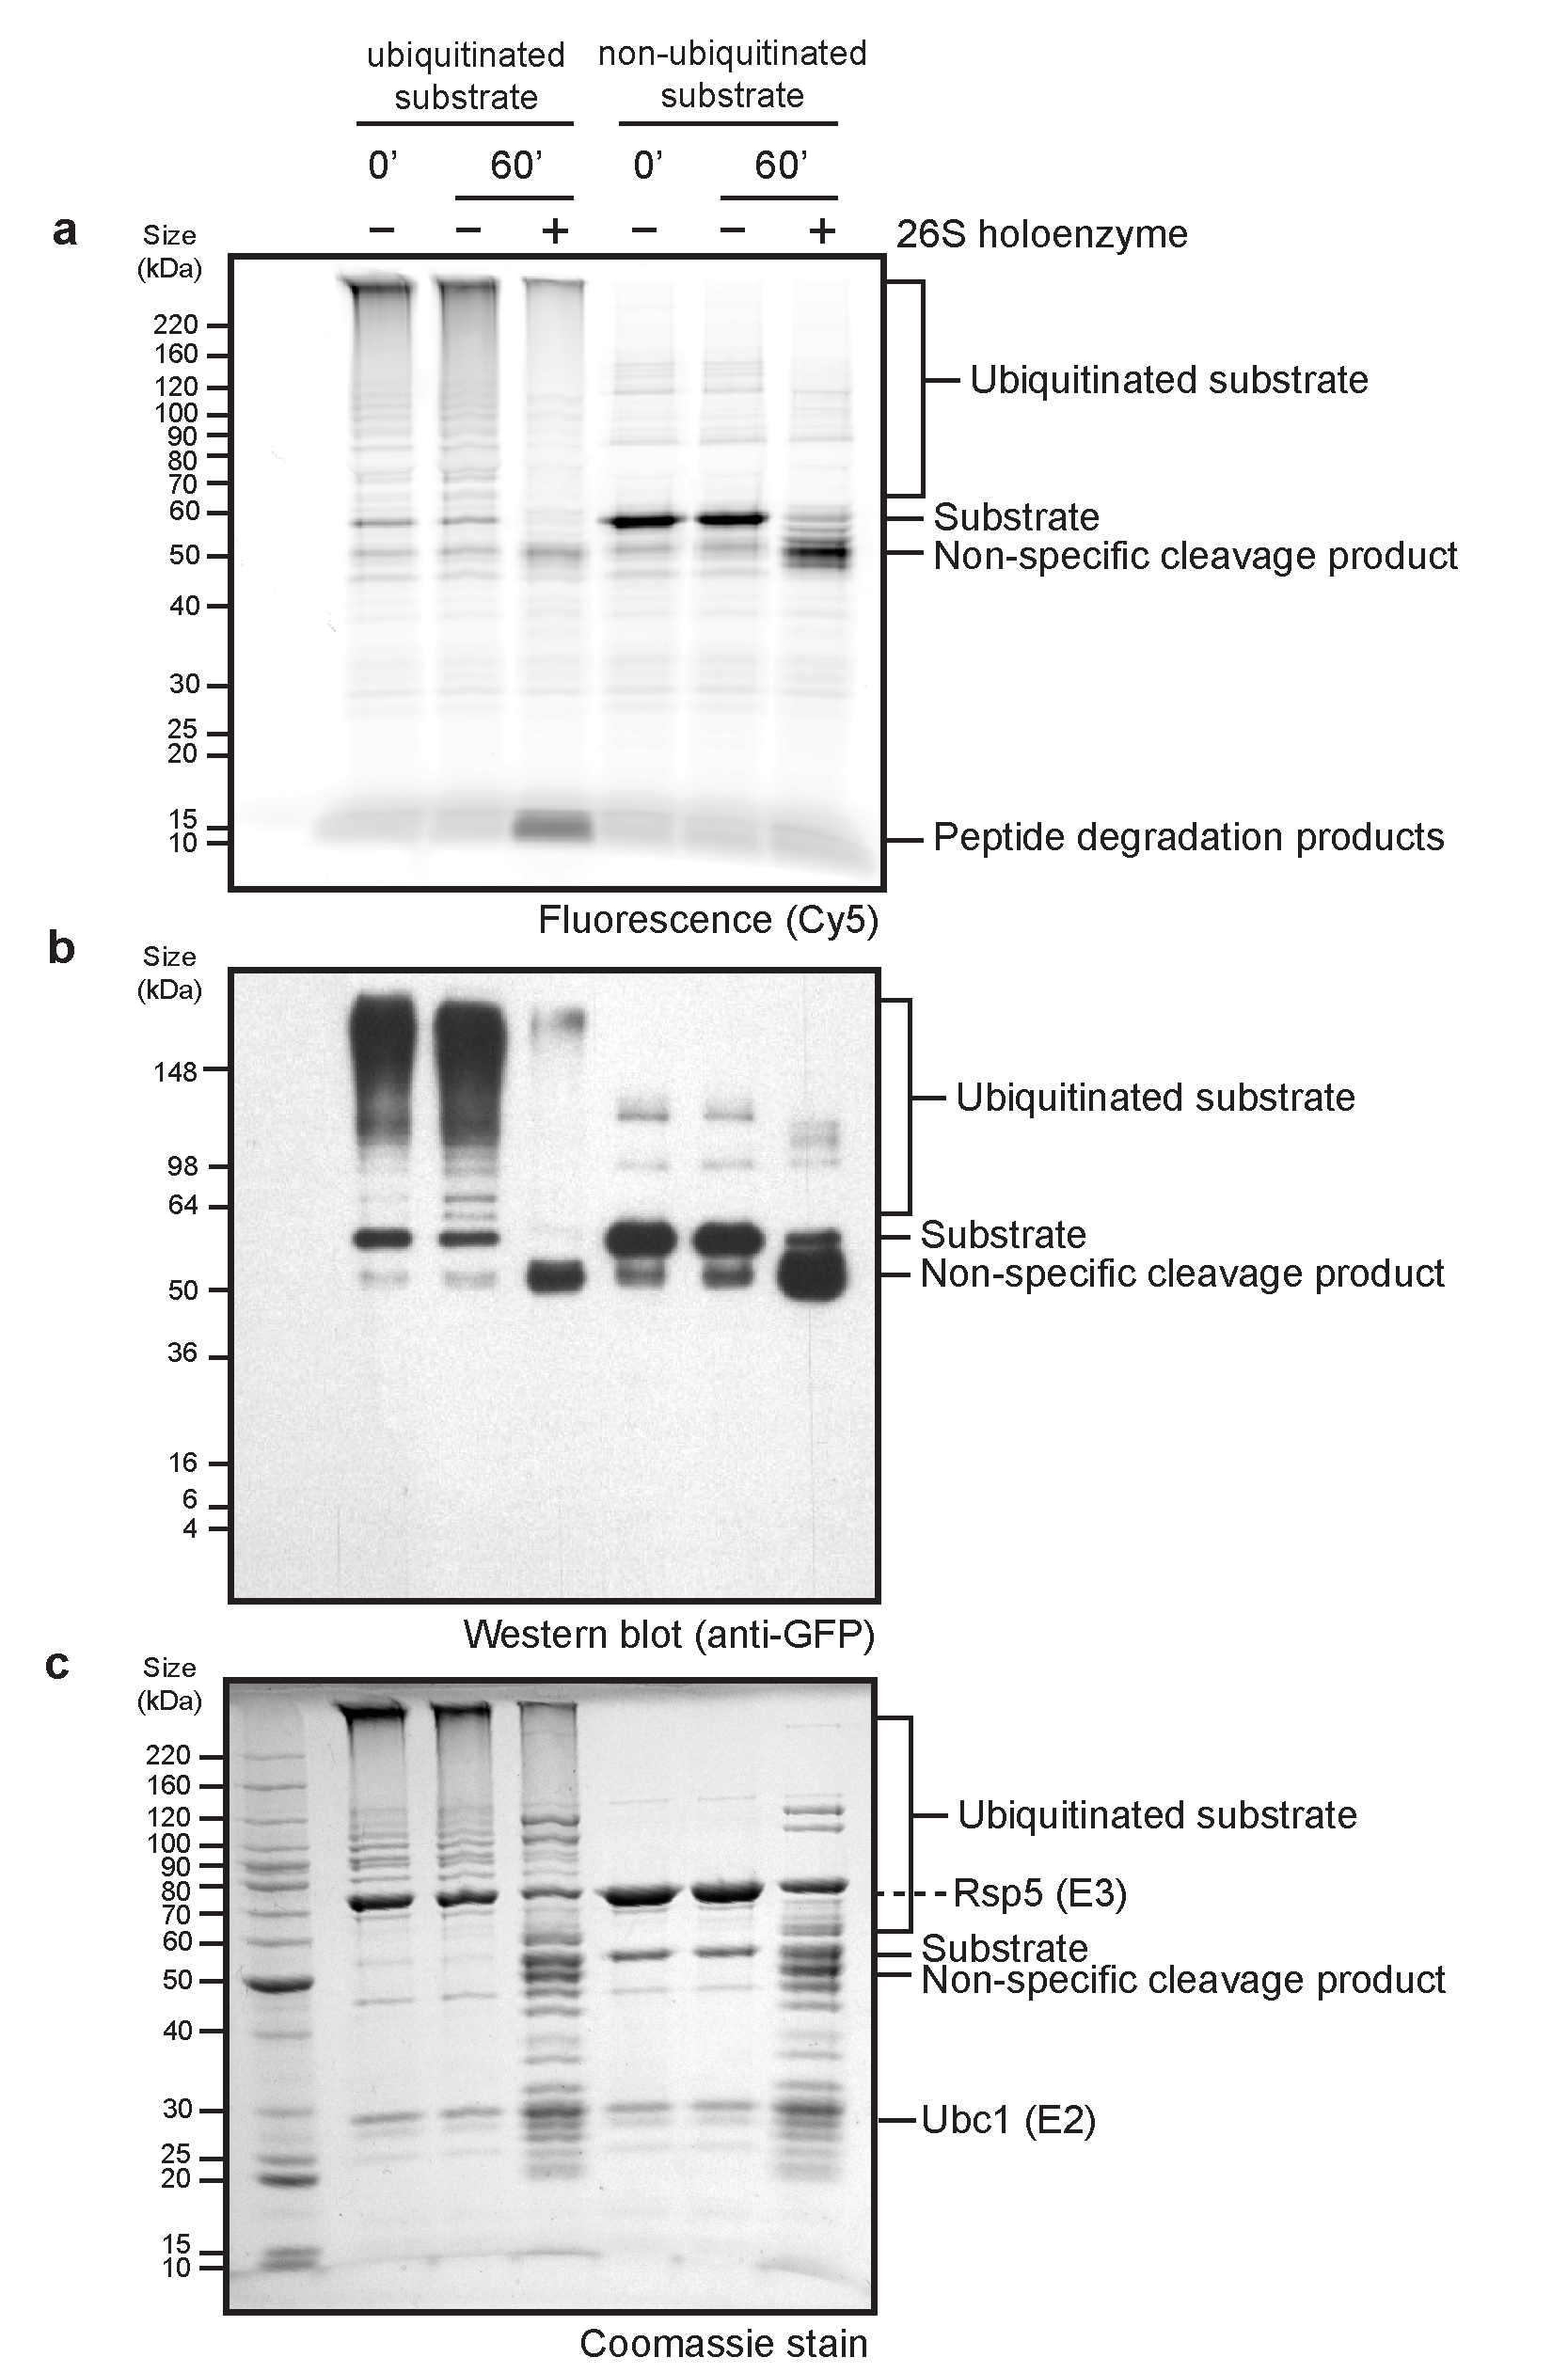
\includegraphics[scale=.45]{gfpdeg}% 
}
\caption[title]{title.\par
The model substrate, a green fluorescent protein (GFP)\---titin$^{V15P}$\---cyclin\---PY fusion, was labeled at the N\---terminus with Cy5 dye and subsequently modified with a polyubiquitin chain \textit{in vitro} using Uba1, Ubc1, Rsp5 and wild\---type ubiquitin.  The non\---ubiquitinated substrate was prepared similarly except wild\---type ubiquitin was omitted from the reaction. Degradation was assessed by incubating substrates with 26S holoenzyme purified from yeast in the presence of an ATP regeneration system at 30�C for one hour.  Substrate degradation was then assessed by running samples on a SDS\---PAGE gel followed by (a) fluorescence scanning to detect the Cy5\---labeled substrate (670 nm band\---pass 30 filter), (b) western blotting using an anti\---GFP antibody, or (c) Coomassie staining for total protein. The fluorescence scan clearly shows the accumulation of small peptide degradation products only for the ubiquitinated substrate in the presence of holoenzyme. Some level of ubiquitin\---independent partial cleavage of an unstructured region of the GFP model substrate was detectable in all three assays. Additional ubiquitination of the substrate was visible in the absence of holoenzyme both by fluorescence scan and anti\---GFP western blot, which was not unexpected as the enzymes used for \textit{in vitro} ubiquitination of the substrate were still present.}
\label{fig:gfpdeg}
\end{figure}

\begin{figure}[p]
\centering
\setlength{\fboxrule}{0pt}
\fbox{%
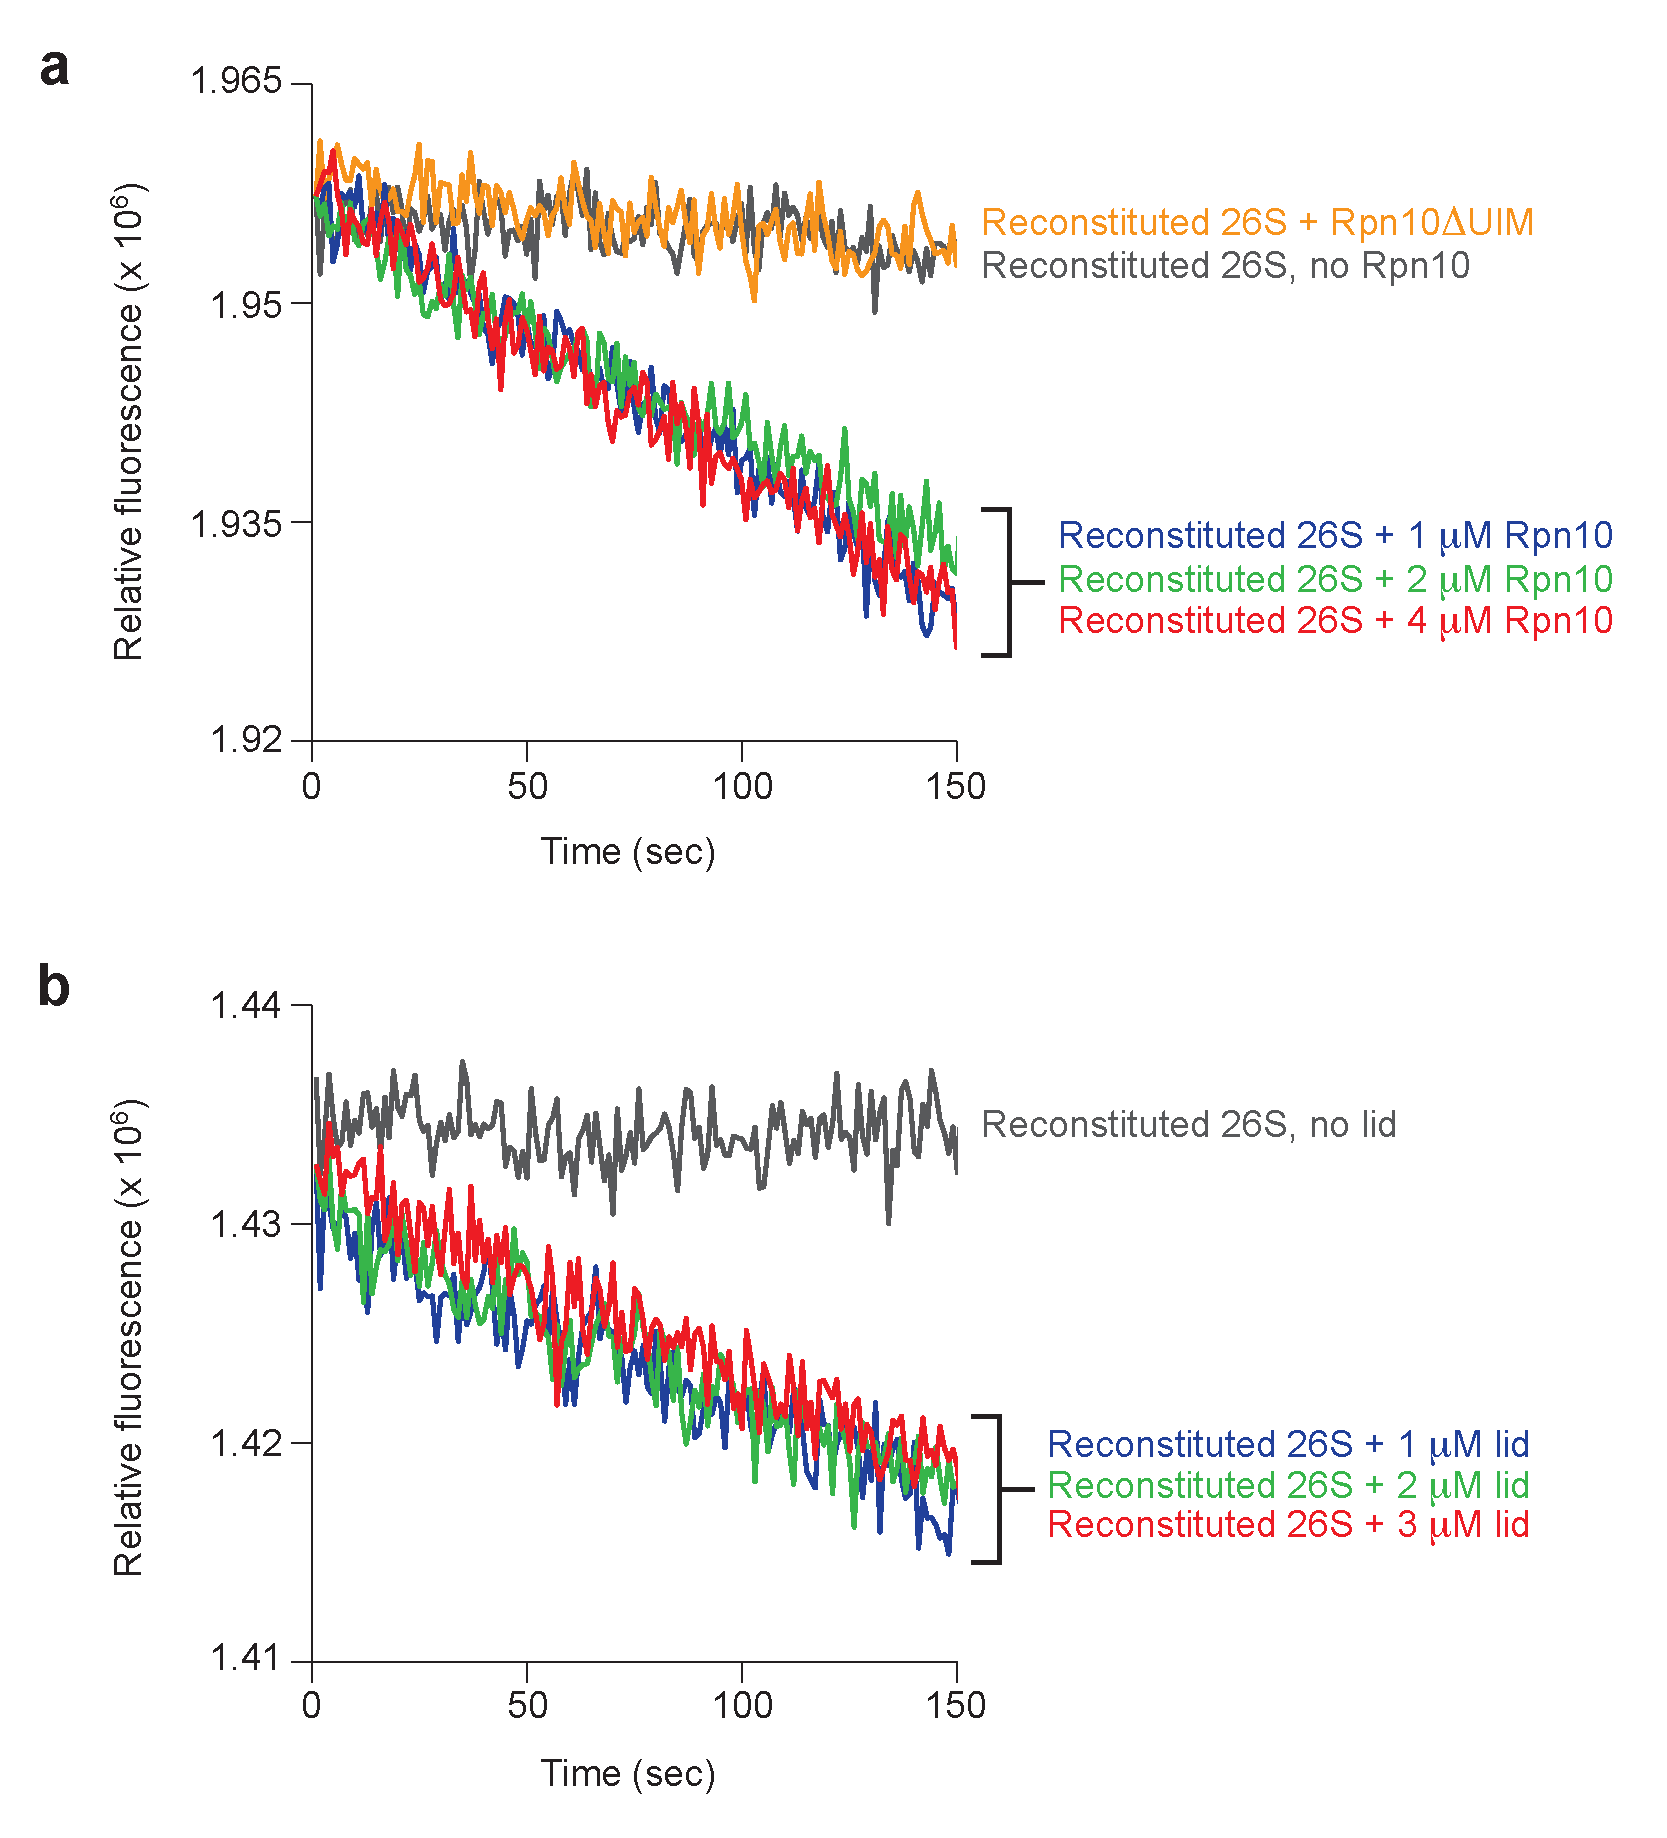
\includegraphics[scale=.5]{degcontrols}% 
}
\caption[Excess lid or Rpn10 do not affect proteasomal degradation]{Excess lid or Rpn10 do not affect proteasomal degradation.\par
Proteasomal degradation was monitored by the decrease in fluorescence of a polyubiquitinated GFP\---fusion substrate (excitation 467 nm, emission 511 nm) upon incubation with reconstituted 26S proteasome. Degradation reactions contained limiting amounts of core particle (yeast) and saturating concentrations of base (\textit{E. coli}\---expressed), lid (yeast), and 1 $\mu$M Rpn10 (\textit{E. coli}\---expressed). To establish that excess amounts of free lid and Rpn10 did not interact with our ubiquitinated substrate and adversely affect the measured degradation rates, we added increasing amounts of (a) Rpn10 or (b) lid and observed that the degradation rate remained constant.}
\label{fig:degcontrols}
\end{figure}






%%-------------------------

\section{Discussion}
alsdjflaksdjflkjdafs

%%-------------------------
\newpage
\vfill

\section{Materials and Methods}

\subsection{Cloning, expression and purification of recombinant base}
Thirteen subunits were cloned into three Novagen vectors including pCOLA\---1 (FLAG\---Rpt1, Rpt2, His$_6$\---Rpt3, Rpt4, Rpt5, Rpt6), pETDuet\---1 (Rpn1, Rpn2, Rpn13), and pACYCDuet\---1 (Nas2, Nas6, Hsm3, Rpn14). Each subunit was preceded by a T7 promoter and all plasmids contained one T7 terminator at the end of the multiple cloning sites. Genes for rare tRNAs were also included in the pACYCDuet\---1 plasmid to account for differences in codon usage between yeast and \emph{E. coli}. Base expression strains were generated by co\---transforming the pETDuet\---1, pCOLA\---1 and pACYCDuet\---1 plasmids into \emph{E. coli} BL21\---star (DE3) cells. The base subcomplex was produced by growing the expression strain to OD600=0.6\---0.8 and inducing with 1mM isopropyl\---b\---D\---thiogalactopyranoside overnight at 18�C. Cells were harvested by centrifugation at 5000 rpm for 15 min, resuspended in nickel buffer (25 mM HEPES pH 7.6, 100 mM NaCl, 100 mM KCl, 10\% glycerol, 10 mM MgCl2, 0.5 mM EDTA, 20 mM imidazole) supplemented with 2 mg ml$^{-1}$ lysozyme, protease inhibitors and benzonase. Cells were lysed by freeze\---thaw and sonication on ice for 1 min 30 sec in 15 sec bursts. Lysate was clarified by centrifugation at 15,000 rpm at 4�C for 30 min. A two\---step affinity purification of the base subcomplex was performed using Ni\---NTA agarose (Qiagen) to select for His$_6$\---Rpt3 and anti\---FLAG M2 resin (Sigma\---Aldrich) selecting for FLAG\---Rpt1. 0.5 mM ATP was present in all purification buffers. The Ni\---NTA and anti\---FLAG M2 columns were eluted with nickel buffer containing 250 mM imidazole or 0.15 mg ml$^{-1}$ 3xFLAG peptide, respectively. The Flag column eluate was concentrated using a 30,000 MWCO concentrator (Amicon) and run on a Superose 6 gel filtration column (GE Healthcare) equilibrated with gel filtration buffer (60 mM HEPES pH 7.6, 50 mM NaCl, 50 mM KCl, 10\% glycerol, 5 mM MgCl2, 0.5 mM EDTA, 1 mM DTT, 0.5 mM ATP).

\subsection{Purification of endogenous yeast complexes}
Yeast holoenzyme, core particle, base and lid subcomplexes were purified from \emph{S. cerevisiae} essentially as previously described61. Frozen yeast cells were lysed using a Spex SamplePrep 6870 Freezer/Mill. Holoenzyme was purified from a yeast strain containing FLAG\---Rpn11. Lysed cells were resuspended in lysis buffer containing 60 mM HEPES pH 7.6, 100 mM NaCl, 100 mM KCl, 10\% glycerol, 5 mM MgCl2, 0.5 mM EDTA, 0.2\% NP\---40 and ATP regeneration mix (5 mM ATP, 0.03 mg ml$^{-1}$ creatine kinase, 16 mM creatine phosphate). Holoenzyme was bound to anti\---FLAG M2 resin and washed with wash buffer (60 mM HEPES pH 7.6, 100 mM NaCl, 100 mM KCl, 10\% glycerol, 5 mM MgCl2, 0.5 mM EDTA, 0.1\% NP-40, 0.5 mM ATP). Holoenzyme was eluted with 0.15 mg ml$^{-1}$ 3xFLAG peptide and further purified by gel filtration using a Superose 6 column with gel filtration buffer (see above). Lid and base subcomplexes were isolated from FLAG\---Rpn11 or FLAG\---Rpn2 yeast strains, respectively, and purified by exposure to a 1 M NaCl wash while bound to anti\---FLAG M2 resin. Base purification buffers included 0.5 mM ATP. Core particle was purified from a 3xFLAG\---Pre1 yeast strain using a 500 mM salt wash. All subcomplexes underwent size exclusion chromatography using a Superose 6 column as described above.

\subsection{Yeast strains}
Yeast lid and holoenzyme were purified from strain YYS40 (genotype MATa ade2\---1 his3\---11,15 leu2\---3,112 trp1\---1 ura3\---1 can1 Rpn11::Rpn11\---3XFLAG(HIS3), source Y. Saeki). Core particle was prepared either from strain RJD1144 (genotype MATa his3\---200 leu2\---3,112 lys2\---801 trp\---63 ura3\---52 PRE1\---FLAG\---6xHIS::Ylpac211(URA3) source R. Deschaies) or strain yAM14 (genotype MATa ade2\---1 his3\---11,15 leu2\---3,112 trip1\---1 ura3\---1 can1\---100 bar1 PRE1::PRE1\---3XFLAG(KanMX), this study).

\subsection{Native gel electrophoresis}
Analysis of proteasome holoenzyme and subcomplexes by native gel was performed as described previously61. Assembly reactions were incubated for 15 min at 23�C with 5 mM ATP, followed by electrophoresis on a 3.5\% native polyacrylamide gel. Electrophoresis was conducted at 4�C with stirring and running buffer containing 0.5 mM ATP. The gel was overlaid with developer solution (running buffer with 100 nM Suc\---LLVY\---AMC peptide (Boston Biochem) and 0.02\% SDS) and incubated at 30�C for 10 minutes prior to imaging. Fluorescence imaging was performed using a Typhoon scanner (GE Healthcare) and followed by Coomassie staining.

\subsection{ATPase and peptidase stimulation assays}
ATPase activity was quantified using an NADH\---coupled ATPase assay. 500 nM base was incubated with 1x ATPase mix (3 U ml$^{-1}$ pyruvate kinase, 3 U ml$^{-1}$ lactate dehydrogenase, 1 mM NADH, 7.5 mM phosphoenol pyruvate) at 30�C. Absorbance at 340 nm was monitored for 900 sec at 10 sec intervals using a UV\---Vis Spectrophotometer (Agilent). Peptidase stimulation was monitored by following the increase in fluorescence resulting from cleavage of a fluorogenic peptide substrate62, Suc\---LLVY\---AMC (Boston Biochem), using a QuantaMaster spectrofluorimeter (PTI). 50 nM core particle was incubated with saturating base subcomplex in the presence of an ATP regeneration system (5 mM ATP, 16 mM creatine phosphate, 6 mg ml$^{-1}$ creatine phosphokinase) and 50 ?M Suc-LLVY-AMC.

\subsection{Fluorescent substrate degradation assay}
Proteasome holoenzyme was reconstituted from core particle, lid, base and Rpn10. A GFP\---titin$^{V15P}$\---cyclin\---PY fusion protein was modified \emph{in vitro} with a polyubiquitin chain using Uba1, Ubc1, Rsp5 and wild-type ubiquitin. Degradation reactions were performed at 30�C in gel filtration buffer (60 mM HEPES pH 7.6, 50 mM NaCl, 50 mM KCl, 10\% glycerol, 5 mM MgCl2, 0.5 mM EDTA, 1 mM DTT, 0.5 mM ATP) supplemented with an ATP regeneration system. Details for the gel-based degradation assay can be found in the legend of Fig. \ref{fig:gfpdeg}. Single and multiple turnover degradation activities were monitored by the loss of GFP fluorescence (excitation 467 nm; emission 511 nm) using a QuantaMaster spectrofluorimeter (PTI). Multiple turnover degradation experiments were performed with 50 nM reconstituted holoenzyme under V$_{max}$ conditions (saturating base, lid and Rpn10) with 2 $\mu$M substrate. Excess base, lid, and Rpn10 did not affect the observed degradation rate (see Fig. \ref{fig:degcontrols} for lid and Rpn10).

%%-------------------------




